


\tikzset{every picture/.style={line width=0.75pt}} %set default line width to 0.75pt        

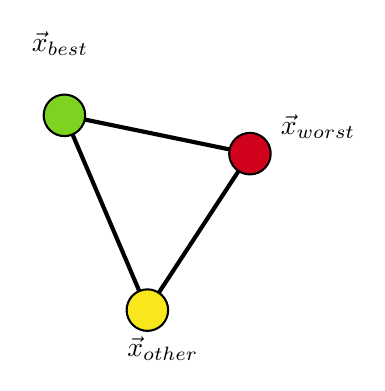
\begin{tikzpicture}[x=0.75pt,y=0.75pt,yscale=-1,xscale=1]
%uncomment if require: \path (0,914); %set diagram left start at 0, and has height of 914

%Straight Lines [id:da0052534278546845226] 
\draw [line width=1.5]    (63.21,89.73) -- (152.59,108.19) ;
%Straight Lines [id:da2220277816214007] 
\draw [line width=1.5]    (103.18,183.58) -- (63.21,89.73) ;
%Straight Lines [id:da006067659711585183] 
\draw [line width=1.5]    (103.18,183.58) -- (152.59,108.19) ;
%Shape: Circle [id:dp15048672252515094] 
\draw  [fill={rgb, 255:red, 126; green, 211; blue, 33 }  ,fill opacity=1 ] (54.01,93.65) .. controls (51.85,88.57) and (54.21,82.7) .. (59.29,80.53) .. controls (64.37,78.37) and (70.25,80.73) .. (72.41,85.81) .. controls (74.57,90.9) and (72.21,96.77) .. (67.13,98.93) .. controls (62.05,101.1) and (56.17,98.73) .. (54.01,93.65) -- cycle ;
%Shape: Circle [id:dp2153424878727488] 
\draw  [fill={rgb, 255:red, 208; green, 2; blue, 27 }  ,fill opacity=1 ] (143.39,112.1) .. controls (141.22,107.02) and (143.59,101.15) .. (148.67,98.99) .. controls (153.75,96.82) and (159.62,99.19) .. (161.79,104.27) .. controls (163.95,109.35) and (161.59,115.22) .. (156.51,117.39) .. controls (151.43,119.55) and (145.55,117.19) .. (143.39,112.1) -- cycle ;
%Shape: Circle [id:dp6498543047529874] 
\draw  [fill={rgb, 255:red, 248; green, 231; blue, 28 }  ,fill opacity=1 ] (93.98,187.49) .. controls (91.82,182.41) and (94.18,176.54) .. (99.26,174.38) .. controls (104.34,172.21) and (110.22,174.58) .. (112.38,179.66) .. controls (114.54,184.74) and (112.18,190.61) .. (107.1,192.78) .. controls (102.02,194.94) and (96.14,192.58) .. (93.98,187.49) -- cycle ;

% Text Node
\draw (46,48) node [anchor=north west][inner sep=0.75pt]   [align=left] {$\displaystyle \vec{x}_{best}$};
% Text Node
\draw (166,88) node [anchor=north west][inner sep=0.75pt]   [align=left] {$\displaystyle \vec{x}_{worst}$};
% Text Node
\draw (92,195) node [anchor=north west][inner sep=0.75pt]   [align=left] {$\displaystyle \vec{x}_{other}$};


\end{tikzpicture}